% !Mode:: "TeX:UTF-8"
%%  本模板推荐以下方式编译:
%%     1. PDFLaTeX[推荐]
%%     2. xelatex [含中文推荐]
%%  注意:
%%  1. 文件默认的编码为 UTF-8 对于windows,请选用支持UTF-8编码的编辑器。
%%   2. 若是模板有什么问题,请及时与我们取得联系,Email:latexstudio@qq.com。
%%   3. 可以到  https://ask.latexstudio.net 提问
%%   4. 请安装 最新版本的 TeXLive 地址:
%%   http://mirrors.ctan.org/systems/texlive/Images/texlive.iso

\documentclass{apmcmthesis}

\usepackage{url}

%%%%%%%%%%%%填写相关信息%%%%%%%%%%%%%%%%%%%%%%%%%%
\tihao{C}                            %选题
\baominghao{apmcm2300201}                 %参赛编号
\begin{document}

\pagestyle{frontmatterstyle}

\begin{abstract}
% using \CJK{UTF8}{gbsn}{Chinese} for Chinese.

New energy vehicles have gained widespread popularity since their introduction, due to their advanced technology, low fuel consumption, and alignment with the global carbon peak and carbon neutrality goals around the world. This paper extensively gathers data on new energy vehicles, traditional fuel-powered cars, and related information. Finally, a series of mathematical models to describe the development of new energy vehicles are established.

For problem 1, 

\textbf{NOTE} that data should be demonstrated here.

For problem 2, 

Ultimately, we provide a summary of the data and mathematical models employed in this study and look ahead to potential future works.


\keywords{New energy vehicles\quad  Keywords2\quad   Keywords3}
\end{abstract}


\newpage
%目录
\tableofcontents


\newpage
\pagestyle{mainmatterstyle}
\setcounter{page}{1}
\section{Introduction}

% 首先写新能源汽车的意义(总体介绍)

% 然后写新能源汽车对中国的特殊意义和在中国的发展
% 以及新能源电动汽车(题目只涉及新能源电动汽车)

% 最后写本文的做法(建模主体即:中国、新能源电动汽车)

New energy vehicles integrate transformative technologies such as new energy sources, new materials, and various disruptive technologies like the internet, big data, and artificial intelligence. This integration propels the transformation of energy, transportation, and information communication infrastructure, fostering an optimized energy consumption structure, elevating the intelligence level of transportation systems and urban operations. This advancement holds significant importance in constructing a clean and beautiful world, and in building a shared future for humanity.

The widespread adoption of new energy vehicles holds particular significance for China. With a large population, China faces substantial carbon emissions from automobiles. The popularization of new energy vehicles will greatly reduce China's energy expenditure and stands as a robust initiative toward achieving ecological civilization.

Within the realm of new energy vehicles, the development of new energy electric vehicles has been particularly rapid. This is primarily due to their low pollution and low energy consumption characteristics. Additionally, new energy electric vehicles typically offer a affordable price, thus enjoying a broad market in China.

This paper collects comprehensive data on China's new energy electric vehicles, including their sales volume, growth rates, traditional car sales, export quantities, and China's policies supporting new energy vehicles. Further, this paper employs methods such as \textbf{xx} and \textbf{xx} to model and analyze the development of China's new energy electric vehicles and their associated impacts.


\section{The Description of the Problem}

In this chapter, we conducted a detailed analysis of six problems related to the development of new energy vehicles and provided approaches to address these problems.

\subsection{Question 1}



\subsection{Question 2}



\subsection{Question 3}



\subsection{Question 4}



\subsection{Question 5}



\subsection{Question 6}




\section{Models}

\subsection{Model for Question 1}

\subsubsection{Terms, Definitions and Symbols}
\% introduce $Terms, Definitions, Symbols$ used in this model.



\subsubsection{Assumptions}


\subsubsection{Data preparation}


\begin{figure}[htbp]
	\centering
	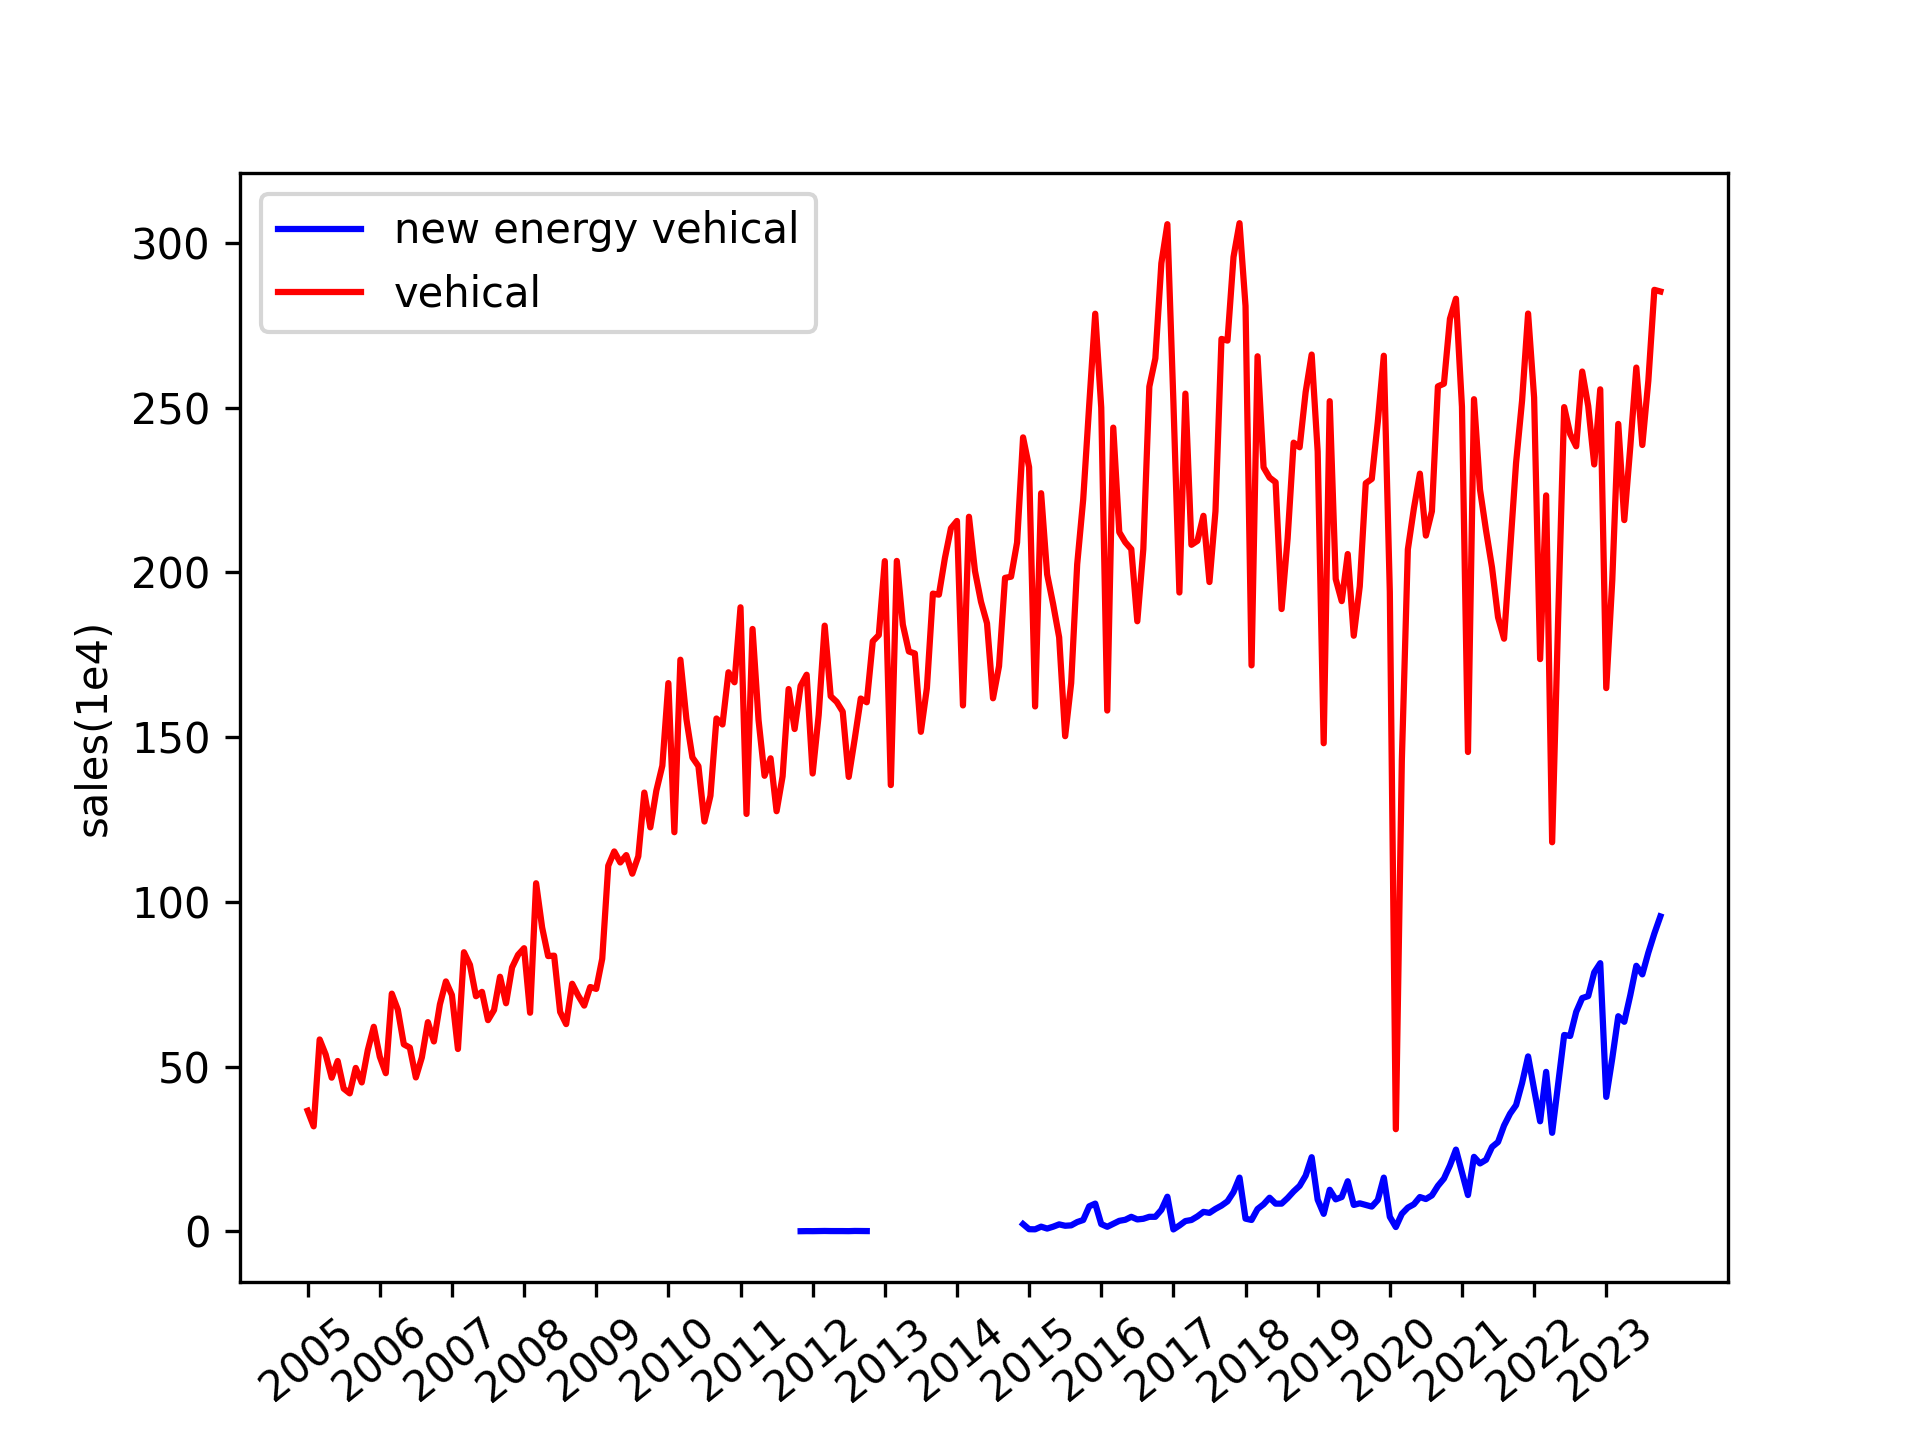
\includegraphics[width=30pc, height=22pc]{origin_new_energy_data}
	\caption{Original data.}
	\label{figure 1}
\end{figure}

\begin{figure}[htbp]
	\centering
	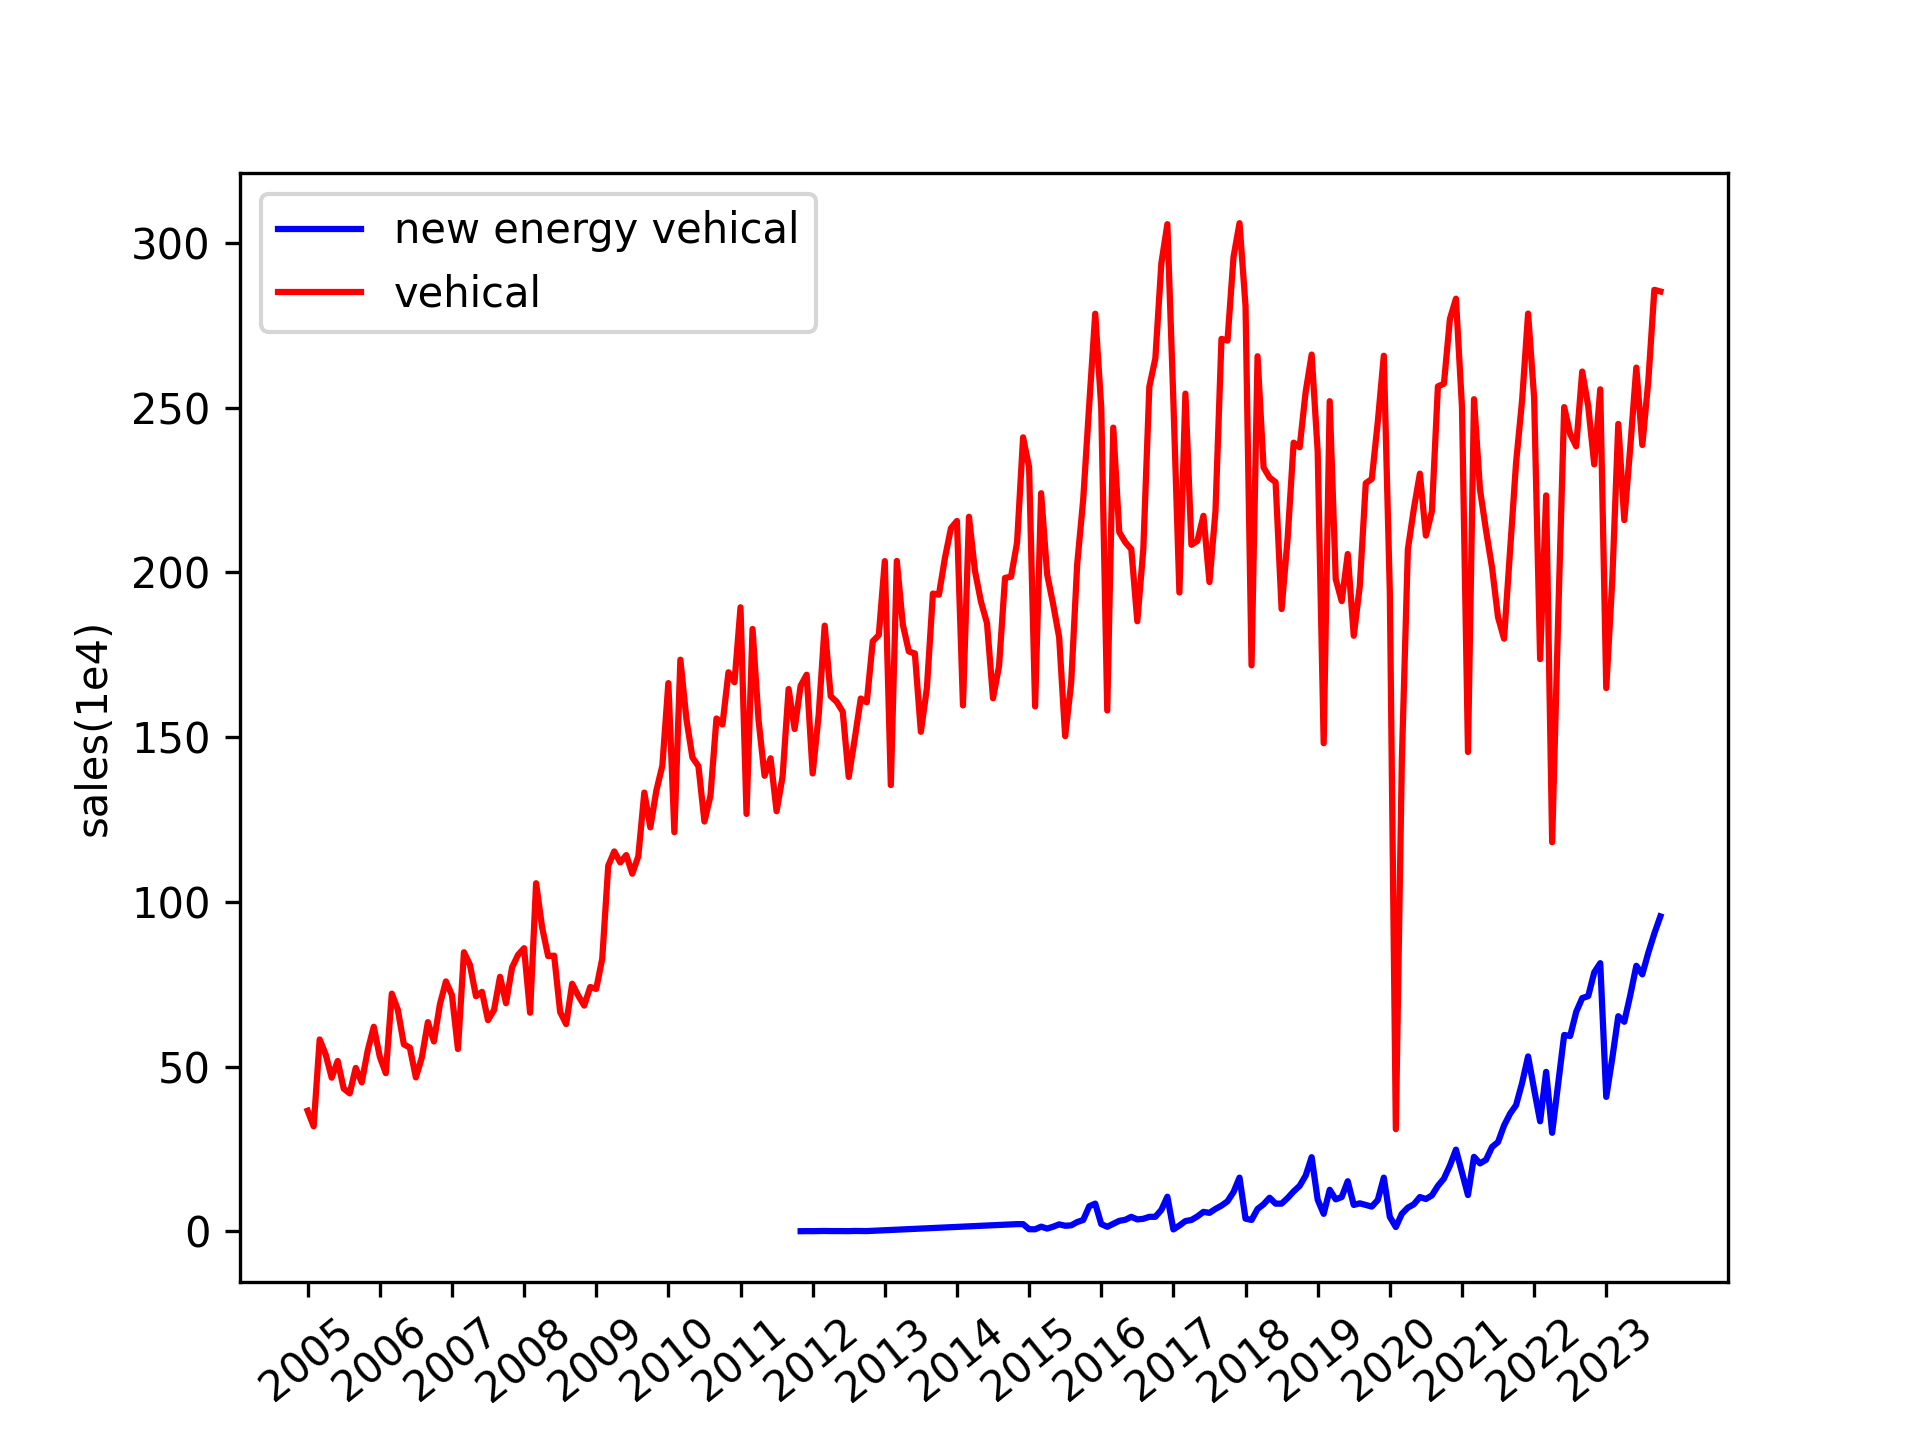
\includegraphics[width=30pc, height=22pc]{interpolated_new_energy_data}
	\caption{Processed data.}
	\label{figure 2}
\end{figure}

\subsubsection{The Foundation of Model}
\% Establish mathematical model here.


\subsubsection{Solution and Result}
\% Solve mathematical model here.


\subsubsection{Analysis of the Result}
\% Conclude here.


\subsubsection{Strength and Weakness}
\% Optional
\begin{description}
\item[Strength:] Strength.
\item[Weakness:] Weakness.
\end{description}


\subsection{Model for Question X}

\subsubsection{Terms, Definitions and Symbols}
\% introduce $Terms, Definitions, Symbols$ used in this model.

\subsubsection{Assumptions}


\subsubsection{Data preparation}


\subsubsection{The Foundation of Model}
\% Establish mathematical model here.


\subsubsection{Solution and Result}
\% Solve mathematical model here.


\subsubsection{Analysis of the Result}
\% Conclude here.


\subsubsection{Strength and Weakness}
\% Optional
\begin{description}
	\item[Strength:] Strength.
	\item[Weakness:] Weakness.
\end{description}


\section{Conclusions}

\subsection{Conclusions of the problem}



\subsection{Methods used in our models}



\subsection{Applications of our models}




\section{Future Work}

\subsection{Advanced models}
\% Optional.\CJK{UTF8}{gbsn}{ 如果希望模型完成更多功能,将期望的功能写在这里,当作对未来模型的展望。}

\subsubsection{model 1}

\subsection{Data collection}
\% Optional.\CJK{UTF8}{gbsn}{ 如果认为可以收集更多样化的数据,可以将期望的数据描述在这里。}

\subsubsection{data 1}




%参考文献
\begin{thebibliography}{9}%宽度9
\bibitem{1} Author, Title, Place of Publication: Press, Year of publication.
\bibitem{2} author, paper name, magazine name, volume number: starting and ending
page number, year of publication.

\end{thebibliography}

\newpage
%附录

\section{Appendix}

\begin{lstlisting}[caption={Data source}]

1. The brands of new energy electric vehicles that hold the largest market share.
http://cpcaauto.com/newslist.php?types=csjd&id=3273

\end{lstlisting}


\end{document} 